\documentclass[tikz]{standalone}
\usetikzlibrary{calc, intersections, math}

\begin{document}
	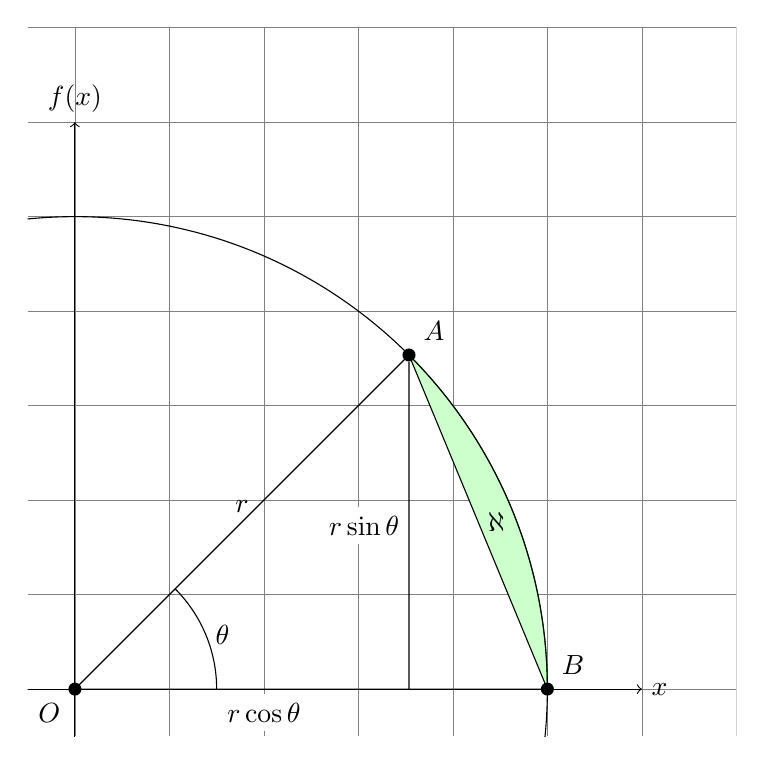
\begin{tikzpicture}[scale=6, mystyle/.style={circle,fill,scale=0.5}]

        % Set the angle of the central arc
		\tikzmath{\angle = 45;}
        
        % selecting the first quadrant
        \clip (-0.1,-0.1) rectangle (1.4,1.4);
        % setting up the Cartesian Grid. Note "help lines" = "gray, very thin"
        \draw[step=.2cm,help lines] (-.1,-.1) grid (2,2);
        % setting up the real and imaginary axis. 
        \draw[->] (-1.5,0) -- (1.2,0) coordinate (x axis) node[right] {$x$};
        \draw[->] (0,-1.5) -- (0,1.2) coordinate (y axis) node[above] {$f(x)$};
		
		% draw and fill the circular segment
		\filldraw[fill=green!20!white, draw=green!50!black, label=$A$] (1cm,0)  arc  (0:\angle:1cm);
		% add the unti circle
		\draw (0,0) circle (1cm);
		% draw and label the central arc AOB
        \draw 
            (0,0) 
                node[mystyle, label=below left:{$O$}] (O) {} -- 
                node[above] {$r$}
            (\angle:1cm) 
                node[mystyle, label=above right:{$A$}] (A) {} -- 
                node[right]{$\aleph$} 
            (0:1cm) 
                node[mystyle, label=above right:{$B$}] (B) {} --
            cycle
                node[pos=.6,fill=white, below,yshift=-.5mm] {$r\cos\theta$};
		% label the central angle
		\draw (0.3,0) arc (0:\angle:0.3) node[midway,right]{$\theta$};
		
        % project a line from A down to the x-axis
        \draw (A) -- node[fill=white, left] {$r\sin \theta$} (A |- x axis);
	\end{tikzpicture}
\end{document}
